\section{图表环境}
\subsection{图片}
普通图片如\autoref{fig:sample}
\begin{figure}[H]
    \centering
    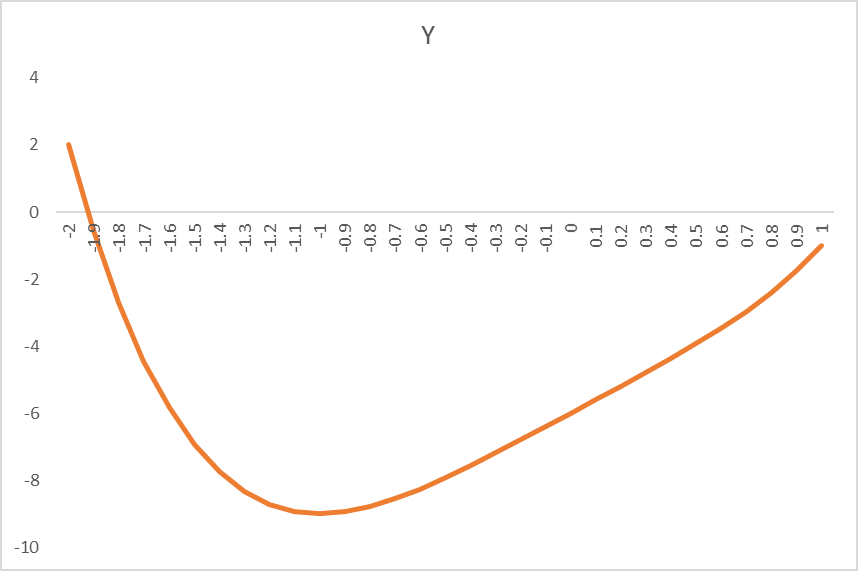
\includegraphics[width=8cm]{sample1.png}
    \caption{Sample Image}
    \label{fig:sample}
\end{figure}

子图环境如\autoref{fig:subfigure},也可以交叉引用子图,如\autoref{fig:subfig_b}

\begin{figure}[H]
    \begin{subfigure}{0.24\linewidth}
        
\includegraphics[width=\textwidth]{a.png}
        \caption{A字母图片}
    \end{subfigure}
    \hfill
    \begin{subfigure}{0.24\linewidth}
        
\includegraphics[width=\textwidth]{b.png}
        \caption{B字母图片}
        \label{fig:subfig_b}
    \end{subfigure}
    \hfill
    \begin{subfigure}{0.24\linewidth}
        
\includegraphics[width=\textwidth]{c.png}
        \caption{C字母图片}
    \end{subfigure}
    \hfill
    \begin{subfigure}{0.24\linewidth}
        
\includegraphics[width=\textwidth]{d.png}
        \caption{D字母图片}
    \end{subfigure}
    \caption{子图示例}
    \label{fig:subfigure}
\end{figure}

\subsection{表格}
\subsubsection{普通表格}
\begin{table}[htbp]
    \centering
    \caption{示例表格}
    \begin{tabular}{rlcc}
        \toprule
        ID & 名称        & 数量 & 单价 \\
        \midrule
        9  & Ruler       & 3    & 1000 \\
        26 & Pen         & 6    & 2000 \\
        32 & \LaTeX Book & 30   & 500  \\
        \bottomrule
    \end{tabular}
    \label{tab:}
\end{table}

\subsubsection{页宽表格}
\begin{table}[!ht]
    \caption{Parameter values}\label{tab:parametervalues}
    \begin{tabular*}{\hsize}{@{}@{\extracolsep{\fill}}ccccccccc@{}}
        \toprule
        &$p_{t}$  &21  &22  &20  &15  &10  &8   &  \\
        \midrule
        &$c_{t}$  &5   &13  &10  &10  &10  &10  &  \\
        &$h_{t}$  &10  &5   &5   &5   &5   &5   &  \\
        &$s_{t}$  &100 &100 &100 &100 &100 &100 &  \\
        &$d_{t}$  &30  &45  &50  &55  &45  &55  &  \\
        \bottomrule
    \end{tabular*}
\end{table}

\autoref{tab:parametervalues}左右都有多余的一列,这样内容能稍微紧凑好看一点。不然的话就是\autoref{tab:parametervalues_}这样

\begin{table}[!ht]
    \caption{Parameter values}\label{tab:parametervalues_}
    \begin{tabular*}{\hsize}{@{}@{\extracolsep{\fill}}ccccccc@{}}
        \toprule
        $p_{t}$  &21  &22  &20  &15  &10  &8     \\
        \midrule
        $c_{t}$  &5   &13  &10  &10  &10  &10    \\
        $h_{t}$  &10  &5   &5   &5   &5   &5     \\
        $s_{t}$  &100 &100 &100 &100 &100 &100   \\
        $d_{t}$  &30  &45  &50  &55  &45  &55    \\
        \bottomrule
    \end{tabular*}
\end{table}

\subsubsection{长表格}

\begin{longtable}{ccccccc}
    \caption{Longtable Caption Here.}                              \\

    \toprule
    ID & Name     & Chinese & Math & English & Physics & Chemistry \\
    \midrule
    \endfirsthead

    \multicolumn{7}{l}{\zihao{6}续上表}                            \\
    \toprule
    ID & Name     & Chinese & Math & English & Physics & Chemistry \\
    \midrule
    \endhead

    \bottomrule
    \multicolumn{7}{r}{\zihao{6}接下表}                            \\
    \endfoot

    \bottomrule
    \endlastfoot
    01 & Percival & 77      & 92   & 92      & 80      & 79        \\
    02 & Ida      & 74      & 87   & 99      & 96      & 73        \\
    03 & Janice   & 71      & 86   & 80      & 99      & 94        \\
    04 & Victor   & 82      & 60   & 100     & 63      & 67        \\
    05 & Oscar    & 61      & 86   & 89      & 100     & 77        \\
    06 & Janice   & 75      & 73   & 86      & 89      & 90        \\
    07 & Lulu     & 90      & 80   & 81      & 63      & 91        \\
\end{longtable}

\subsubsection{表格中含有图片}

\begin{table}[!ht]
    \centering
    \caption{table captoin here.}
    \begin{tabular}{ccc}
        \toprule
        Index    & Fig.A & Fig.B \\
        \midrule
        Pictures &
        \begin{minipage}[b]{0.12\columnwidth}
            \centering
            \raisebox{-0.5\height}{
\includegraphics[width=\linewidth]{a.png}}
        \end{minipage}
                 &
        \begin{minipage}[b]{0.12\columnwidth}
            \centering
            \raisebox{-0.5\height}{
\includegraphics[width=\linewidth]{b.png}}
        \end{minipage}
        \\
        \bottomrule
    \end{tabular}
\end{table}

\subsubsection{表格过宽}
表格过宽的第一反应一定是:这个表的形式是否正确,这个表放在这里是否真的有必要。如果确实有必要再用如下方法调整其宽度。

\begin{table}[!ht]
    \centering
    \caption{过宽表格}
    \resizebox{\linewidth}{!}{
        \begin{tabular}{ccc}
            \toprule
            变量              & 单位 & 描述                                                                                   \\
            \midrule
            $l_\textup{very}$ & m    & 这是一个很长很长很长很长很长很长很长很长很长很长很长很长很长很长很长很长很长很长的变量 \\
            \bottomrule
        \end{tabular}
    }
    \label{tab:toowide}
\end{table}

\subsubsection{过宽长表格}
这种更极端,更要首先考虑是否有必要。附录里放数据用用还可以。

思路:longtable是不兼容resizebox的,所以只能调小字号,使得宽度合适
{
\zihao{-6}
% \resizebox{\linewidth}{!}{
\begin{longtable}{clc ccc ccc ccc cc}
    \caption{6月部分小区二手房详细数据}                                                                                                               \\
    \hline
    行政区     & 小区名称     & 编号 & 建筑年龄 & 建筑面积 & 装修    & 绿化率  & 容积率  & 物业费  & 停车位  & 地铁数  & 购物中心 & 学校    & 医院    \\
    \hline
    \endfirsthead
    \multicolumn{14}{l}{\zihao{7}续上表}                                                                                                              \\
    \hline
    行政区     & 小区名称     & 编号 & 建筑年龄 & 建筑面积 & 装修    & 绿化率  & 容积率  & 物业费  & 停车位  & 地铁数  & 购物中心 & 学校    & 医院    \\
    \hline
    \endhead
    \hline
    \multicolumn{14}{r}{\zihao{7}接下表}                                                                                                              \\
    \endfoot
    \hline
    \endlastfoot

    未央区     & 恒大名都     & 1    & -0.4175  & 0.7360   & 0.4137  & 1.0222  & -0.047  & -0.1416 & -0.3166 & 0.4048  & -0.2817  & 0.8421  & 1.2480  \\
               & 华宇时间城   & 2    & -0.62    & -0.0419  & -1.5722 & -0.478  & -0.1422 & -0.1416 & 0.4742  & -1.3096 & 0.6402   & 0.0443  & -1.1705 \\
               & 西派国际     & 3    & -1.0249  & -0.3269  & -3.5582 & -0.478  & 0.3266  & 3.6994  & 0.0788  & -0.1667 & 0.0256   & 0.3102  & 0.6899  \\
               & 金桥太阳岛   & 4    & 1.6069   & -0.0276  & 0.4137  & 0.2721  & 0.0336  & -0.1416 & -0.3166 & 0.4048  & -1.8183  & 0.5762  & 0.8760  \\
    雁塔区     & 海伦国际     & 5    & -0.0127  & -0.1594  & -1.5722 & -0.478  & -0.5891 & 0.5058  & 0.4742  & 0.4048  & -1.2036  & 0.0443  & -0.0543 \\
               & 金裕花园     & 6    & 2.0118   & -1.3598  & 0.4137  & -2.7283 & 0.9127  & -0.789  & -0.712  & 0.4048  & -0.8963  & 0.5762  & 0.5039  \\
               & 豪盛时代华城 & 7    & 1.4044   & -1.4784  & 0.4137  & 1.0222  & 0.0336  & 0.5058  & -0.1848 & -0.7381 & -1.2036  & 1.108   & 1.2480  \\
               & 绿地与湖     & 8    & -0.8224  & -0.7383  & 0.4137  & -0.1779 & 0.7808  & 0.5058  & 1.1332  & -0.7381 & 0.9475   & 0.5762  & -1.7286 \\
\end{longtable}
}
% }